\chapter{\ifproject%
\ifenglish Project Structure and Methodology\else โครงสร้างและขั้นตอนการทำงาน\fi
\else%
\ifenglish Project Structure\else โครงสร้างของโครงงาน\fi
\fi}

\qquad ในบทนี้จะกล่าวถึงเนื้อเรื่องของเกม, เกมเพลย์, วิธีการเล่นเกม เพื่อให้ผู้เล่นได้เข้าใจเป้าหมายและวิธีการเล่นของเกมนี้มากยิ่งขึ้น

% \makeatletter

% % \renewcommand\section{\@startsection {section}{1}{\z@}%
% %                                    {13.5ex \@plus -1ex \@minus -.2ex}%
% %                                    {2.3ex \@plus.2ex}%
% %                                    {\normalfont\large\bfseries}}

% \makeatother
% %\vspace{2ex}
% % \titleformat{\section}{\normalfont\bfseries}{\thesection}{1em}{}
% % \titlespacing*{\section}{0pt}{10ex}{0pt}

\section{เนื้อเรื่อง}

\qquad เกมมีเนื้อเรื่องเกี่ยวกับ ในป่าแห่งหนึ่งที่มีสองเผ่าที่อาศัยอยู่ร่วมกัน คือเผ่า Doggy และเผ่า Kitty ในอดีตทั้งสองเผ่าอยู่ร่วมกันอย่างสันติ โดยที่แบ่งปันทรัพยากรซึ่งกันและกัน 
แต่แล้วในทั้ง 2 เผ่า ก็เกิดมีผู้ไม่พอใจ อยากให้เผ่าตัวเองได้ทรัพยากรที่มากกว่า ไม่อยากแบ่งทรัพยากรให้อีกเผ่าได้ใช้ ทั้ง 2 เผ่าเริ่มแก่งแย่งทรัพยากรกันเกิดเป็นสงครามระหว่าง 2 เผ่าเรื่อยมา

\section{Gameplay}

\qquad ก่อนเริ่มเกมผู้เล่นจะสามารถสุ่มหรือเลือกเผ่าของตัวเองได้ เมื่อเริ่มเกมแล้วผู้เล่นจะถูกสุ่มตําแหน่งฐานหลักของตัวเอง 
โดยที่ในเกมจะมีทรัพยากรเริ่มต้นให้ผู้เล่นคือ ฐานหลักที่ใช้สร้าง unit พื้นฐาน, unit พื้นฐาน, อาหาร (Food), ไม้ (Wood) 
ที่สามารถนําไปใช้สร้าง unit และ building ได้

\begin{figure}[h]
  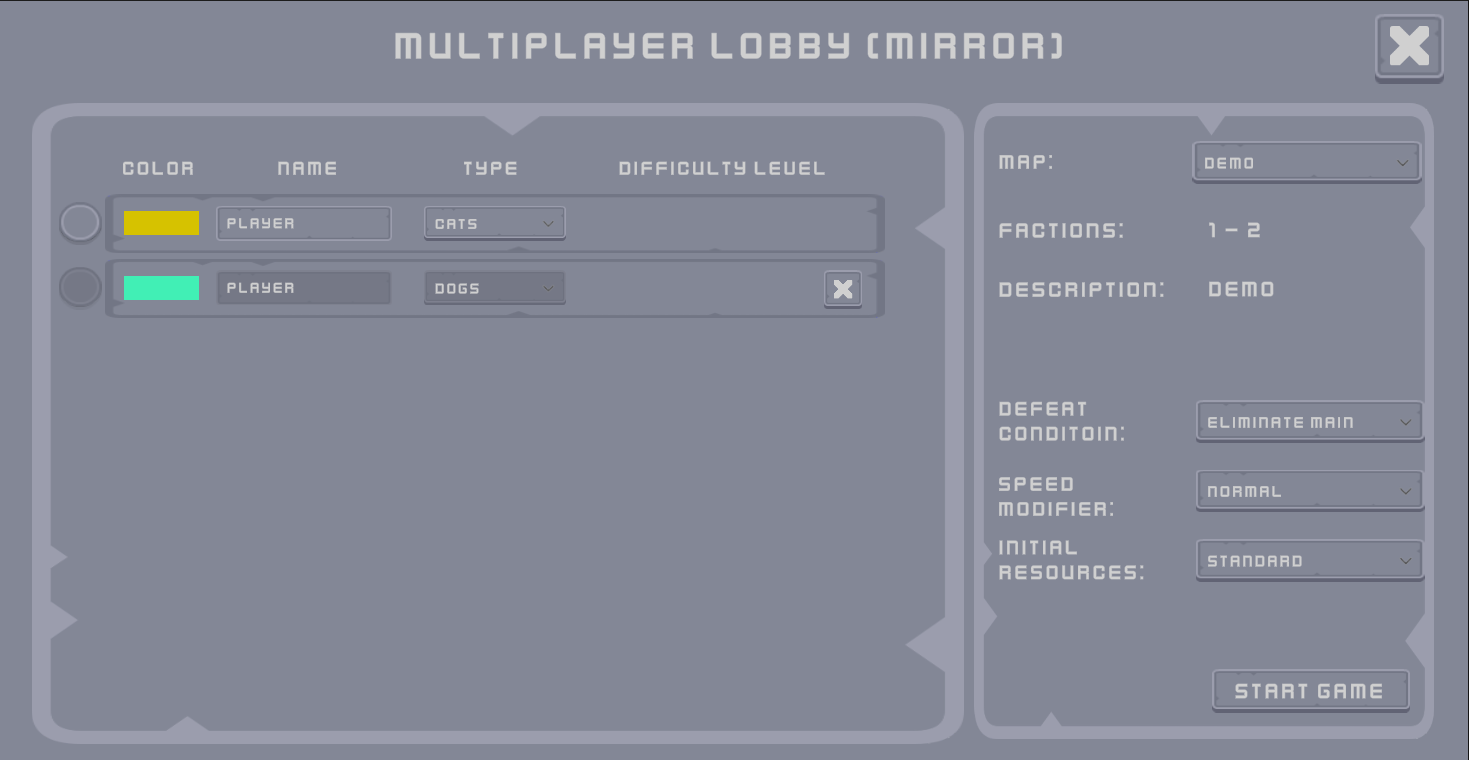
\includegraphics[width=\linewidth]{joingamePage.png}
  \caption{หน้าเลือกเผ่าก่อนเริ่มเกม}
\end{figure}

\begin{figure}[h]
  
\includegraphics[width=\linewidth]{resource.png}
  \caption{Resource Bar}
\end{figure}

\enskip แต่ละเผ่าจะมีทรัพยากรพิเศษที่สามารถนําไปใช้ในการสร้าง Hero (unit พิเศษ) ได้ สําหรับเผ่า Doggy คือ กระดูก (Bone) ส่วนของเผ่า Kitty คือ ก้างปลา (Fishbone) ซึ่งทรัพยากรพิเศษทั้งสองนี้จะสุ่มวางตาม
พื้นที่ต่างๆ

\enskip ในการเล่นผู้เล่นจะต้องสร้าง unit พื้นฐานเพื่อใช้ในการเก็บรวบรวมทรัพยากร (Food, Wood, Bone/Fishbone)
นํามาสร้างสิ่งก่อสร้างต่างๆซึ่งใช้ในการสร้าง unit ต่อสู้แต่ละแบบและอัญเชิญ Hero ของฝั่งตัวเอง 
เพื่อที่ผู้เล่นจะได้ตั้งกองกําลังและนําไปบุกหรือตั้งรับฝั่งตรงข้าม

\enskip การสร้าง unit ของแต่ละฝั่งนั้นมีการสร้างได้จํานวนจํากัดผู้เล่นต้องทําการสร้างสิ่งก่อสร้าง 
นั่นก็คือ บ้าน เพื่อที่จะขยาย capacity ซึ่งมี limit ของการขยายอยู่ด้วย

\enskip เงื่อนไขในการชนะหรือแพ้ คือการที่ผู้เล่นฝั่งใดฝั่งหนึ่งสามารถทําลายฐานหลักของอีกฝั่งได้

\begin{figure}[ht]
  \centerline{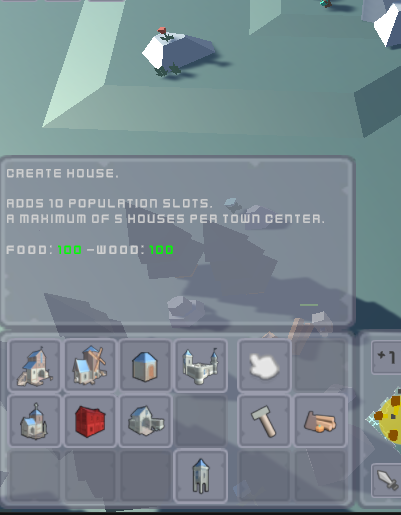
\includegraphics[scale=.7]{createBuilding.png}}
  \caption{แสดงเมนูการสร้าง building ของ unit พื้นฐาน}
\end{figure}

\begin{figure}[h]
  \centerline{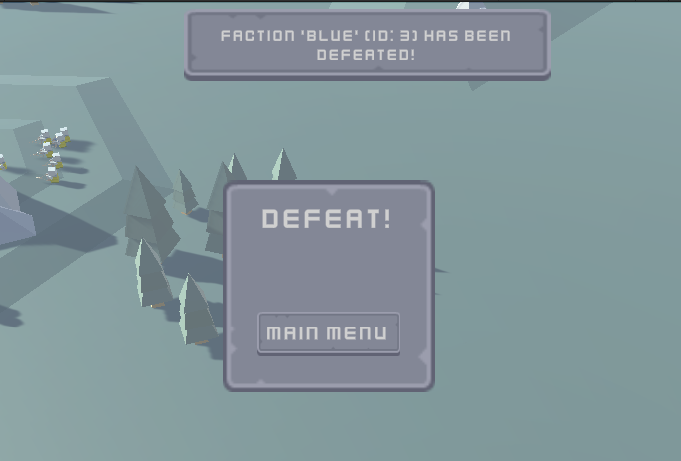
\includegraphics[scale=.6]{result.png}}
  \caption{แสดผลชนะ/แพ้ เมื่อทำลาย/ถูกทำลายฐานหลัก}
\end{figure}
\subsection{ระบบภายในเกม}

\begin{itemize}
  \item ระบบการสร้าง unit
  
  \qquad ในฐานหลักนั้นจะมีระบบการสร้างตัว unit พื้นฐานที่สามารถนําไปเก็บรวบรวมทรัพยากรได้ 
  และมีสิ่งก่อสร้างอื่นที่สามารถสร้าง unit ประเภทอื่นได้ เช่น Barrack สำหรับการสร้าง unit ต่อสู้
  \item ระบบสร้างสิ่งก่อสร้าง (building)
  
  \qquad ในการสร้างสิ่งก่อสร้าง จะให้ผู้เล่นใช้ตัว unit พื้นฐานในการสร้างสิ่งก่อสร้าง ซึ่งสิ่งก่อสร้างบางชนิดจะมีเงื่อนไขที่ต้องสร้างสิ่งก่อสร้างบางประเภทก่อนถึงจะทําการสร้างสิ่งก่อสร้างนั้นได้
  \item ระบบการต่อสู้
  
  \qquad ผู้เล่นสามารถทําการควบคุม unit ต่อสู้ / Hero เพื่อนําไปต่อสู้กับฝั่งตรงข้าม
  \item ระบบ Fog of War
  
  \qquad ใน map จะมีระบบซ่อนข้อมูลบนแผนที่ (Fog of War) ซึ่งทําให้ผู้เล่นต้องทําการสํารวจเพื่อเปิดเผยพื้นที่
  \item ระบบอัพเกรด unit
  
  \qquad ในเกมจะมีสิ่งก่อสร้างที่สามารถอัพเกรดตัว unit ต่อสู้ได้
  \item ระบบการขยาย capacity
  
  \qquad ผู้เล่นต้องทําการสร้างก่อสร้าง “บ้าน” เพื่อเพิ่มความจุในการสร้าง unit โดยรวมได้
\end{itemize}